\documentclass[british,format=acmlarge,screen=true,anonymous=false,review=false]{acmart}

\usepackage[l2tabu,orthodox]{nag}
\usepackage{fixltx2e}
\usepackage{babel}
\usepackage[iso]{isodate}
\usepackage[utf8]{inputenc}
\usepackage[T1]{fontenc}
\usepackage{xspace}

%\usepackage{mathpazo}
%\usepackage[scaled=0.95]{helvet}
\usepackage{courier}

\usepackage{graphicx}
%\usepackage{hyperref}
\usepackage[missing=0.9.12]{gitinfo}

\usepackage{fpmacros}
\usepackage{idrislang}
\usepackage{url}
\usepackage{natbib}

%\input{conf.ltx}
\input{library.ltx}

\title{State Machines All The Way Down}
\subtitle{An Architecture for Dependently Typed Applications}

\author{Edwin Brady}
\affiliation{
\institution{University of St Andrews}
\department{School of Computer Science}
\city{St Andrews}
\country{Scotland}
}
\email{ecb10@st-andrews.ac.uk}

\newcommand{\states}{\texttt{ST}}

\begin{abstract}
    A useful pattern in dependently typed programming is to define a state
    transition system, for example the states and operations in a network
    protocol, as an indexed monad.  We index each operation by its input
    and output states, thus guaranteeing that operations satisfy pre- and
    post-conditions, by typechecking.  However, what if we want to write a
    program using several systems at once?  What if we want to define a high
    level state transition system, such as a network application protocol, in
    terms of lower level states, such as network sockets and mutable variables?

    In this paper, we present an architecture for dependently typed
    applications based on a hierarchy of state transition systems, implemented
    in a generic data type \states{}. This is based on a monad
    indexed by \emph{contexts} of resources, allowing us to reason about
    multiple state transition systems in the type of a function.
    Using \states{}, we show: how to implement a state transition system as a
    dependent type, with type level guarantees on its operations; how to
    account for operations which could fail; how to
    \emph{combine} state transition systems into a larger system; and, how to
    implement larger systems as a hierarchy of state transition systems.
    We illustrate the system by implementing a number of examples, including a
    graphics API, POSIX network sockets, asynchronous programming with threads,
    and a high level network application protocol.
\end{abstract}


\begin{document}
\bibliographystyle{ACM-Reference-Format}
\citestyle{acmauthoryear}

\maketitle

\section{Introduction}

Software relies on state, and many components rely on state machines. For
example, they describe network transport protocols like TCP~\citep{rfc793}, and
implement event-driven systems and regular expression matching.
%
Furthermore, many fundamental resources like network sockets and
files are, implicitly, managed by state machines, in that certain
operations are only valid on resources in certain states, and those operations
can change the states of the underlying resource.  For example, it only makes
sense to send a message on a connected network socket, and closing a socket
changes its state from ``open'' to ``closed''. State machines can also encode
important security properties. For example, in the software which implements
an ATM, it's important that the ATM dispenses cash only when the machine is
in a state where a card has been inserted and the PIN verified.

Despite this, state transitions are generally not checked by compilers.
We routinely use type checkers to ensure that variables and
arguments are used consistently, but statically checking that
operations are performed only on resources in an appropriate state is not well
supported by mainstream type systems.
%
In this paper, we show how to represent state machines precisely in the
dependently typed programming language Idris~\citep{brady2013idris},
and present a library which allows composing larger programs from multiple
state transition systems. The library supports composition in two ways:
firstly, we can use several independently implemented state transition
systems at once; secondly, we can implement one state transition system
in terms of others.

%inspired by the work of Hancock and Setzer on describing
%interactive programming in dependent type theory with command and response
%trees~\citep{hancock-interactive}, and by ongoing work on algebraic effects and
%handlers~\citep{Plotkin2009,Bauer}.  

A motivation for this work is to be able to define communicating
systems, where the type system verifies that each participant follows a 
defined protocol. This is inspired by Session Types~\citep{Honda93,Honda08},
in which the state of a session at any point represents the allowed
interactions on a communication channel. 
%One of the goals, therefore,
%is to represent a form of session types using dependent types. 

However, in order to use session types effectively in practice, we need to be
able to use them in larger systems, interacting with other components. The
\states{} type we present in this paper will allow us to implement a system as
a hierarchy of state machines, and as an example we will implement a
client-server system in which a client requests a random number within a
specific bound from a server, and in which the server processes requests
\emph{asynchronously}. All of the examples are available
online (for review: submitted as supplementary material).

\subsection{Contributions}

We build on previous work on algebraic effects in
Idris~\citep{brady-eff2013,brady-tfp14}. 
In this earlier work, an \emph{effect} is described by an algebraic data
type which gives the operations supported by that effect, and which
is parameterised by a \emph{resource} type.
Operations can change the types of those resources, meaning
that we can implement and verify state transition systems using effects.
However, there are shortcomings: the concrete resource type is defined by the
\emph{effect signature} rather than by its \emph{implementation}; 
it is not possible to create \emph{new} resources in a
controlled way; and, it is not possible to implement \emph{handlers} for
effects in terms of other effects.
%
In this paper, we address these shortcomings, making the following
specific contributions:

\begin{itemize}
\item We present a type, \states{}, which allows a programmer to 
describe a the pre- and post-conditions of a stateful function, creating
and destroying resources as necessary (Section~\ref{sect:statemachines}).
\item We describe the implementation of \states{}, in particular using
Idris' proof automation to construct proofs of correct state management
without programmer intervention (Section~\ref{sect:implementst}).
\item We show how to use \states{} to describe existing stateful APIs,
notably working with network sockets, and to implement high level stateful
systems, such as network application protocols, in terms of these lower level
systems (Section~\ref{sect:examples}).
\end{itemize}

An important goal of \states{} is \emph{usability}. Concretely, this means
that the types need to be readable and need to help direct a programmer to a
working implementation, and error messages need to explain problems clearly. 
We therefore use holes (Section~\ref{sect:getdata})
to help build programs interactively type level programming
(Section~\ref{sect:sttype}) to provide a readable type level notation, and
error reflection (Section~\ref{sect:errorreflection}) to rewrite error messages
into the language of the problem domain.

Using \states{}, we can encode the assumptions we make about state transitions
in a type, and ensure that these assumptions hold at
run time. Moreover, by allowing state machines to be composed both horizontally
(using multiple state machines at once within a function) and vertically
(implementing a state machine in terms of other, lower level, state machines),
\states{} provides an \emph{architecture} for larger scale dependently typed
programs.

%\subsection{Motivation: Client-Server Communication}

%\label{sect:motivating}

% For each state machine, we use the type system to guarantee that operations
% satisfy their necessary \emph{preconditions}, for example that we can only send
% a reply to a message after receiving a request.  To begin, therefore, 
% we will describe how to represent a state machine in a type, including error
% handling, for a small example: a data store which will only allow data
% to be read after a user has logged in.

\section{Example: A data store, requiring a login}

Our goal is to use the type system not only to describe the inputs
and outputs of functions precisely, but also to explain the effect of
functions on any external resources. 
One way to achieve this is to use an indexed monad~\citep{atkey-param},
where for each operation the monad supports, the type carries a
\remph{precondition} which must hold before the operation is executed,
and a \remph{postcondition} which holds after the operation is executed,
possibly depending on the result of the operation. In a sense, these
are Hoare triples~\citep{hoarelogic}, embedded in the type.
%
In this section, we introduce this idea with a small example: a data store which requires users
to log in before giving access to secret data. 

\subsection{State Transitions in the Store}

The store has two states:
\texttt{LoggedIn}, which means that a user is logged in and able to access
data; and \texttt{LoggedOut}, which means that the user is not logged in.
Reading data is only allowed when the system is in the \texttt{LoggedIn} state.
%
Figure~\ref{fig:login} illustrates the data store, showing the
\remph{states} the system can be in (\texttt{LoggedOut} and \texttt{LoggedIn})
and the operations a user can perform on the system. The operations are:

\begin{itemize}
\item \texttt{login}, which is valid when the system is in the 
\texttt{LoggedOut} state, and either results in the system being in the
\texttt{LoggedIn} state, if login was successful, or the \texttt{LoggedOut}
state otherwise (for example, due to an incorrectly entered password).
\item \texttt{logout}, which is valid when the system is in the
\texttt{LoggedIn} state, and moves the system to the \texttt{LoggedOut} state.
\item \texttt{readSecret}, which returns the data held in the store, and
is only valid when the system is in the \texttt{LoggedIn} state.
\end{itemize}

\begin{figure}[h]
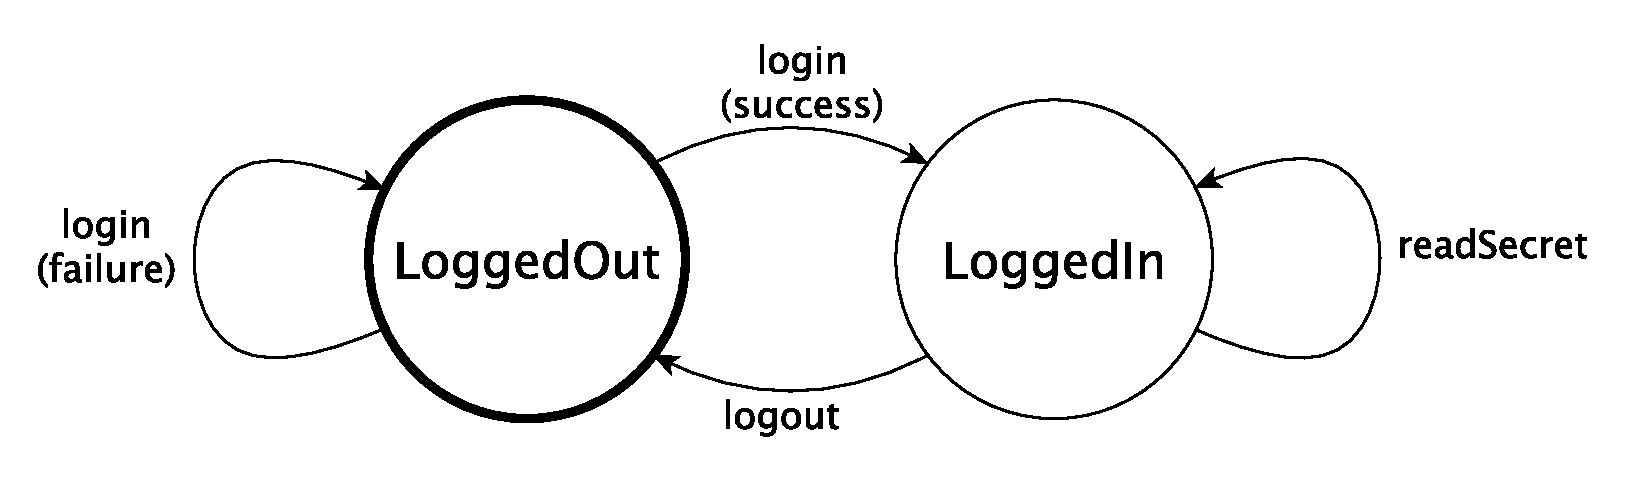
\includegraphics[width=10cm]{diagrams/login.pdf}
\caption{A state machine describing the states and transitions in a system
which allows a program to read some secret data only after successfully logging
in to a data store.}
\label{fig:login}
\end{figure}

By using the type system to capture the state of this system, we can be
sure that a program will only succeed in reading data when it has successfully
logged in to the system. 

\subsection{Representing State Transitions in a Type}

Our goal is that attempting to read data without logging in should result in a
static type error.  Listing~\ref{fig:storemonad} shows how we can achieve this
using an indexed monad.

\small
\begin{code}[float=h, frame=single,caption={Implementing the state store as
an indexed monad},label=fig:storemonad]
data Access = LoggedOut | LoggedIn
data LoginResult = OK | BadPassword

data Store : (ty : Type) -> Access -> (ty -> Access) -> Type where
     Login : Store LoginResult LoggedOut
                   (\res => case res of
                                 OK =>          LoggedIn
                                 BadPassword => LoggedOut)
     Logout :     Store ()     LoggedIn  (const LoggedOut)
     ReadSecret : Store String LoggedIn  (const LoggedIn)

     Pure : (x : ty) -> Store ty (st x) st
     Lift : IO ty -> Store ty st (const st)
     (>>=) : Store a st1 st2 -> ((x : a) -> Store b (st2 x) st3) -> Store b st1 st3
\end{code}
\normalsize

The \texttt{Store} indexed by the type of the result of the operation, the
required input state, and an output state calculated from the result of the
operation. In the simplest cases, such as \texttt{Logout}, the result has no
influence on the result, so we use \texttt{const} (which returns its first
argument and discards its second) to compute the result state:

\small
\begin{code}
Logout : Store () LoggedIn (const LoggedOut)
\end{code}
\normalsize

When we \texttt{Login}, on the other hand, the result state depends on the
result of the operation. If login is successful, it returns \texttt{OK},
and the resulting state of the system is \texttt{LoggedIn}; otherwise, it
is \texttt{LoggedOut}:

\small
\begin{code}
Login : Store LoginResult LoggedOut (\res => case res of
                                                  OK =>          LoggedIn
                                                  BadPassword => LoggedOut)
\end{code}
\normalsize

\subsection{Implementing a program to access the \texttt{Store}}

\label{sect:getdata}

Listing~\ref{fig:storeprog} shows how to combine operations on the store into a
complete function which attempts to login, then reads and prints the data if
successful, or prints an error if not.

\small
\begin{code}[float=h, frame=single,caption={A function which logs in to the
store and reads the secret data if login succeeds},label=fig:storeprog]
getData : Store () LoggedOut (const LoggedOut)
getData = do result <- Login
             case result of
                  OK => do secret <- ReadSecret
                           Lift (putStr ("Secret: " ++ show secret ++ "\n"))
                           Logout
                  BadPassword => Lift (putStr "Failure\n")
\end{code}
\normalsize

Rather than writing \texttt{getData} in one go, we develop it interactively
using \emph{holes}. The following listing contains a hole
\texttt{getData\_rest}, which stands for the rest of the sequence after
attempting to login:

\small
\begin{code}
getData : Store () LoggedOut (const LoggedOut)
getData = do result <- Login
             ?getData_rest
\end{code}
\normalsize

Then, if we check the type of the hole, we can see both the current state of
the system explicitly in the type, and the required state at the end of the
function. Here, we see we need to inspect \texttt{result}:

\small
\begin{code}
getData_rest : Store () (case result of
                              OK => LoggedIn
                              BadPassword => LoggedOut) (const LoggedOut)
\end{code}
\normalsize

%The type here indicates that we can only make progress 
%by inspecting the value of \texttt{result}.
%Functions with holes can be type checked, and even compiled, although
%executing an incomplete program gives a run time error.

We leave \remph{execution} of a \texttt{Store} program abstract her;
this dependis on factors such as how to connect to the store, the security
policy, and so on.
Nevertheless, by defining an indexed monad for the operations on a data store,
we can be sure that programs which access the store correctly follow a protocol
of logging in before reading data. However, there are limitations to this
approach. For example:

\begin{itemize}
\item What if we want to write programs which use other external 
resources, as well as the data store?
\item % What if we need access to several different stores? 
Can we connect to an arbitrary number of stores, rather than being limited to
one?
\item \texttt{Store} describes a session with a
\remph{connected} store. How do we handle connecting and disconnecting?
\end{itemize}

In the rest of this paper, we will decribe a library, \states{}, written in
Idris, which allows us to describe APIs such as those provided by
\texttt{Store}.  It will address the above limitations, allowing us to
\remph{compose} multiple stateful systems, implement systems in terms of other,
lower level systems, and create and destroy resources as required.

\endinput

\endinput

\begin{figure}
\begin{center}
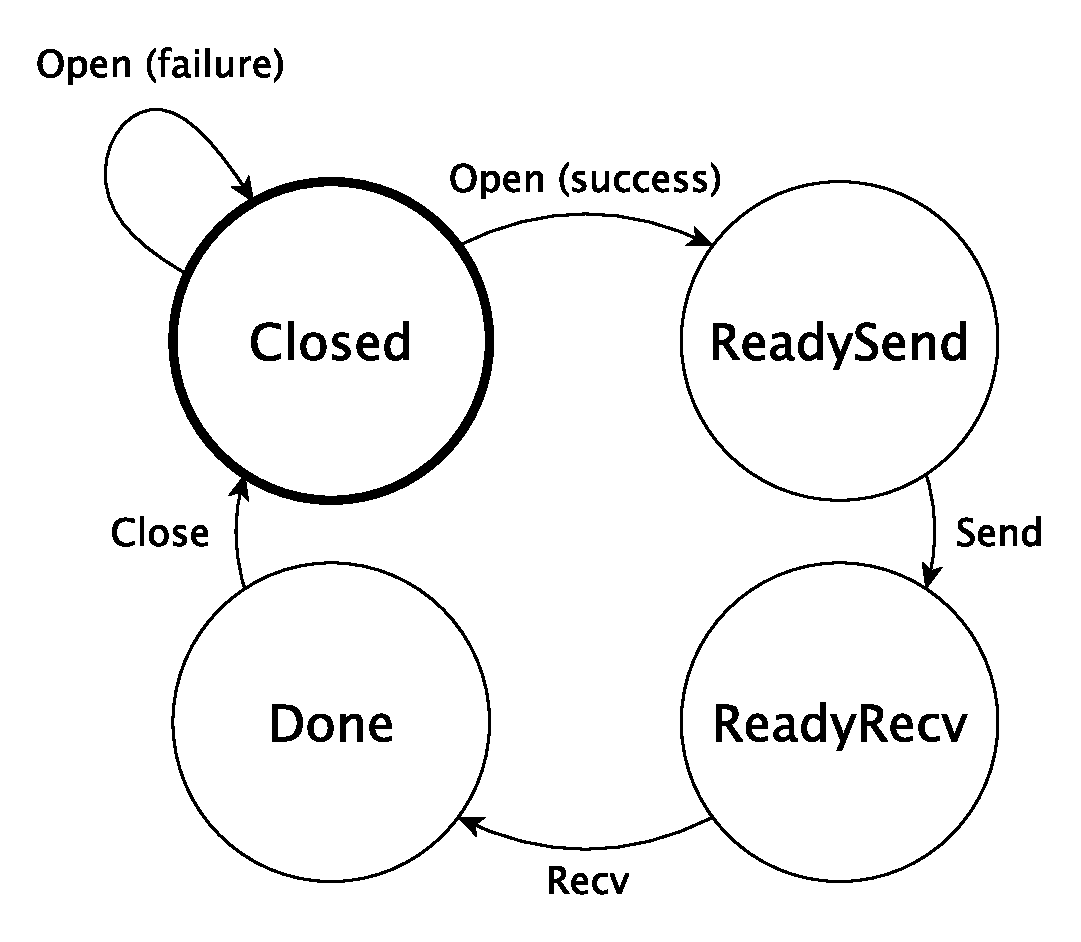
\includegraphics[width=7cm]{diagrams/randclient.pdf}
\end{center}
\caption{A state transition diagram which shows the states and
operations of a client which connects to a server, sends a single message
    and receives a reply. The initial and final state is \texttt{Closed}.}
\label{fig:randclient}
\end{figure}

Figure~\ref{fig:randclient} shows the general form of the states in a
client, where the client connects to a server, sends a message, waits for
a reply, then closes the connection.
Connecting to the server may fail, for example due to a network error, so
in practice we'll need to check whether the \tFN{Open} operation was
successful. Furthermore, although we may have implemented the client
correctly, we can't assume that the server is implemented correctly. If the
server is following a different protocol, \tFN{Recv} may also fail.

\begin{figure}
\begin{center}
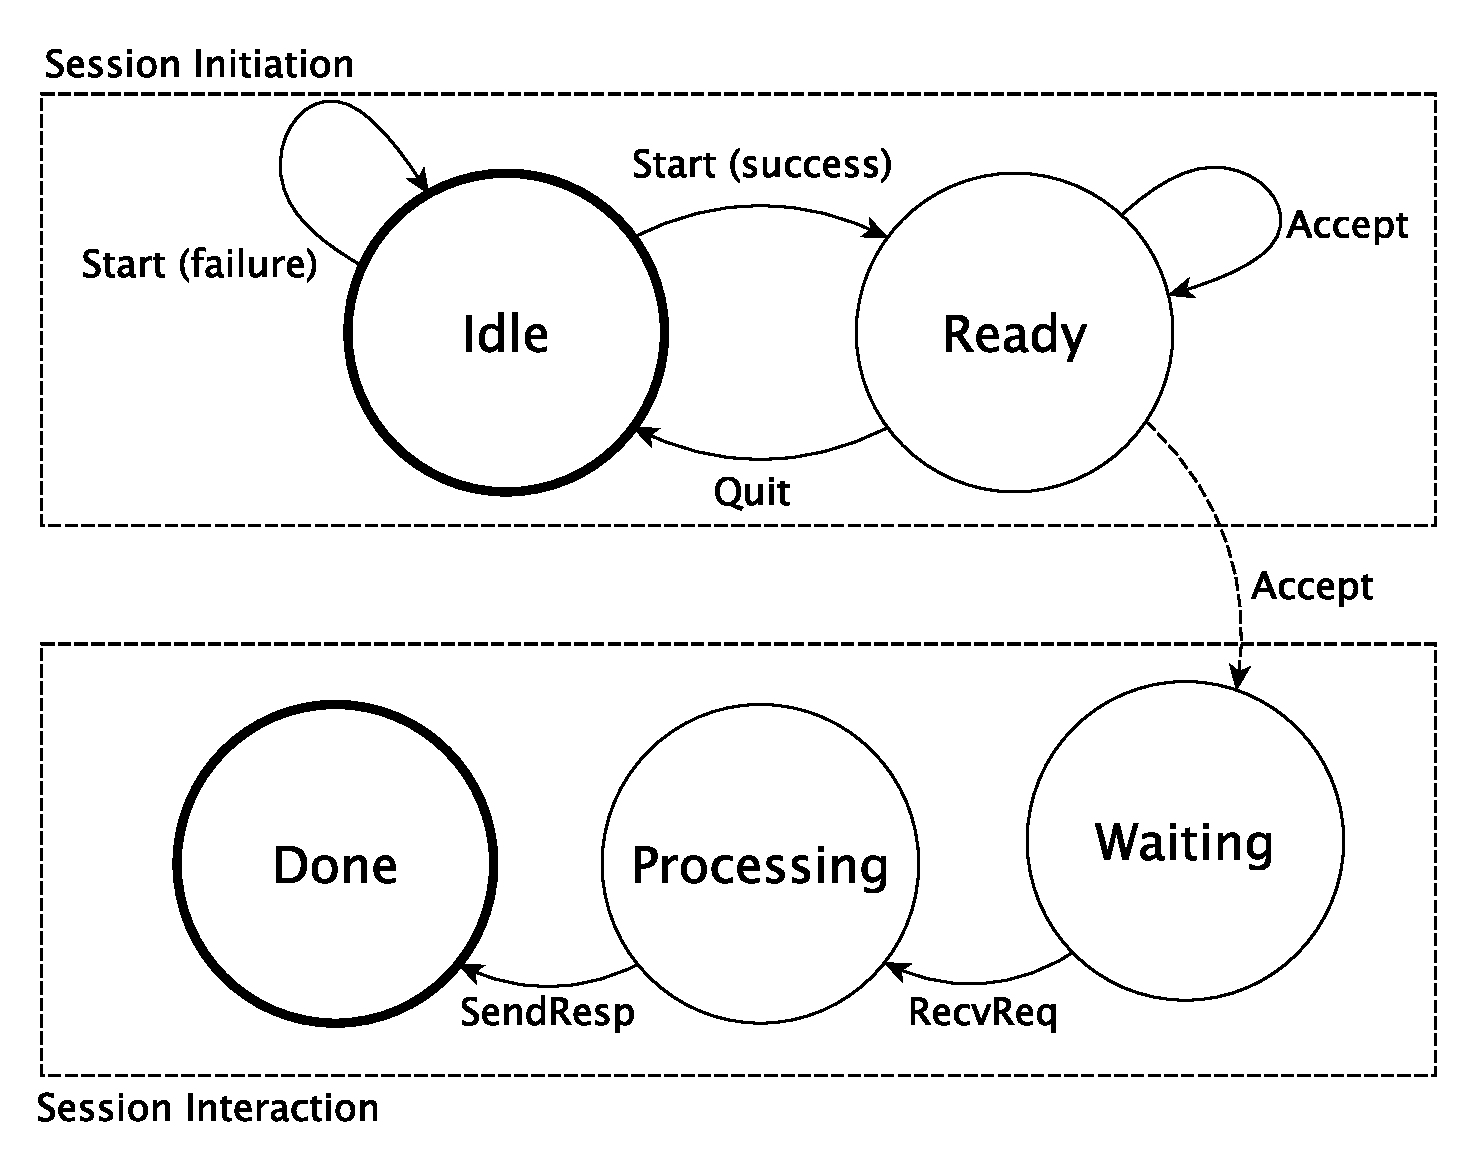
\includegraphics[width=9cm]{diagrams/randserver.pdf}
\end{center}
\caption{A state transition diagram which shows the states and
operations of a server which waits for connections from a client.
    On accepting a connection, it also starts a new machine in the \texttt{Waiting}
    state. The initial state is \texttt{Idle} and the final states are
    \texttt{Idle} and \texttt{Done}.}
\label{fig:randserver}
\end{figure}

A client only has to deal with one connection, to a single server. A server, on
the other hand, may receive requests from several clients. 
Figure~\ref{fig:randserver} shows the general form of the states in a server
which waits for connections from clients, and on receiving a connection
initiates a session in which it waits for an incoming message, then sends
a reply. When it initiates a session, the session itself might run in 
another thread or process. There are two state machines here:

\begin{enumerate}
\item \textbf{Session initiation:} either the server is not running, or it's ready
for an incoming connection. When it receives an incoming connection, it
sets up a new \emph{session interaction} state machine for that connection
and continues waiting for connections
\item \textbf{Session interaction:} the session waits for an incoming message,
processes that message and sends a response, then the session is complete
\end{enumerate}


%\section{Type-level State Machines}

\label{sect:motivate}


\section{\states{}: Describing state transitions in types}

\label{sect:statemachines}

In this section, we introduce the \states{} library. It is built around
an indexed monad \texttt{STrans} which allows us to
compose several stateful systems such as the \texttt{Store}.
We will see how to describe \remph{interfaces}
of stateful systems, how to provide \remph{implementations} of those interfaces
which work in a particular monad, then how to combine multiple stateful
systems in one program. Finally, we will introduce \texttt{ST}, a top level
type which allows us to describe the behaviour of a program in terms of a list
of \emph{state transitions}. 
%In this section, we focus on how to 
%\emph{use} \texttt{STrans} and \texttt{ST}; in the next, we will look in more
%detail at its implementation.

\subsection{Generalising Stateful Programs: Introducing \texttt{STrans}}

\label{sect:strans}

We would like to \remph{generalise} the approach taken in defining
\texttt{Store} to support \remph{multiple} state transition systems at once,
and use types to describe not only the transitions in individual systems,
but also to describe when new systems are \remph{created} and
\remph{destroyed}. 
Furthermore, to be accessible to developers and practitioners, we aim to
provide a \remph{readable} API with helpful error messages.
To summarise, we have the following high level requirements:

\begin{itemize}
\item Types should capture the \remph{states} of resources. That is,
they should:
describe \remph{when} operations are valid; and,
describe \remph{how} the results of operations affect resources.
\item We should be able to use multiple stateful interfaces together. That is,
stateful APIs shold \remph{compose}.
\item Types should be \remph{readable}, and clearly express the behaviour
of operations.
\item Error messages should clearly describe when an operation violates
the protocol given by the type.
\end{itemize}

The \states{} library is built around the following indexed monad, which
describes sequences of state transitions and expresses in its type
how the state transitions affect a collection of resources:

\small
\begin{code}
data STrans : (m : Type -> Type) -> (ty : Type) ->
              (in_ctxt : Context) -> (out_ctxt : ty -> Context) -> Type
\end{code}
\normalsize

The indices of \texttt{STrans} are:

\begin{itemize}
\item \texttt{m} --- an underlying monad, in which the stateful program
is to be executed
\item \texttt{ty} --- the result type of the program
\item \texttt{in\_ctxt} --- an \remph{input context}; a list
of variables and their states \remph{before} the program is executed
\item \texttt{out\_ctxt} --- an \remph{output context}, calculate from the
result of the program, consisting of a list of variables and their states
\remph{after} the program is executed.
\end{itemize}

The input and output contexts correspond to the
\texttt{Access} parameters of \texttt{Store}, except that they store
\remph{lists} of a variable name paired with a type, which
reflect the current state of a \remph{resource}.
For example, a \texttt{Context} which contains a reference to a logged out
data store and a file open for reading could be written as follows:

\small
\begin{code}
[store ::: Store LoggedOut, handle ::: File Read]
\end{code}
\normalsize

The names \texttt{store} and \texttt{handle} here are labels, of a type
\texttt{Var} defined by \texttt{ST}, and are used to refer to specific states
inside an \texttt{STrans} function. The idea, overall, is that we define
\remph{interfaces}\footnote{An interface in Idris is, essentially, like a type
class in Haskell, with some minor differences which do not concern us in this
paper.} which describe operations for creating, modifying and updating
resources as \texttt{STrans} programs. 

\small
\begin{code}[float=h, frame=single,caption={An interface for the data
store, using \texttt{STrans} to describe the state transitions in each
operation},label=fig:storestrans]
interface DataStore (m : Type -> Type) where
  Store : Access -> Type

  connect : STrans m Var [] (\store => [store ::: Store LoggedOut])
  disconnect : (store : Var) -> STrans m () [store ::: Store LoggedOut] (const [])

  login : (store : Var) ->
          STrans m LoginResult 
                   [store ::: Store LoggedOut]
          (\res => [store ::: Store (case res of
                                          OK => LoggedIn
                                          BadPassword => LoggedOut)])
  logout : (store : Var) ->
           STrans m () [store ::: Store LoggedIn]
                (const [store ::: Store LoggedOut])
  readSecret : (store : Var) ->
               STrans m String [store ::: Store LoggedIn]
                        (const [store ::: Store LoggedIn])
\end{code}
\normalsize

Listing~\ref{fig:storestrans}
shows how we can define an interface which supports access to a data
store, like the \texttt{Store} indexed monad we defined in the previous
section.
%
In addition to operations for logging in and out, and reading the secret
from the server, this interface provides two further operations for
connecting to and disconnecting from a store:

\begin{itemize}
\item \texttt{connect} begins with no resources available and returns a new
variable. The output context states that the variable refers to a store
in the \texttt{LoggedOut} state:

\small
\begin{code}
connect : STrans m Var [] (\store => [store ::: Store LoggedOut])
\end{code}
\normalsize

\item \texttt{disconnect}, given a resource which \remph{must} be in the
\texttt{LoggedOut} state, removes that resource:

\small
\begin{code}
disconnect : (store : Var) ->
             STrans m () [store ::: Store LoggedOut] (const [])
\end{code}
\normalsize

\end{itemize}

The interface is parameterised by an underlying monad, \texttt{m}.  To
implement this interface\footnote{In Haskell terms, this would mean providing
an instance of the class.}, as we will do in Section~\ref{sect:implstore}, we
need to explain how to implement the operations in a specific monad. 

As before, the types of \texttt{login}, \texttt{logout} and \texttt{readSecret}
explain how the operations affect a state, but now we provide a label
\texttt{store} which refers to a specific state in the \texttt{Context}.
Furthermore, by encapsulating the operations in an interface, we can
constrain the types of functions to allow access to only the interfaces
we need. Listing~\ref{fig:storegetdata} shows how to implement
\texttt{getData} in this setting. 
This also uses a \texttt{ConsoleIO} interface which provides operations
\texttt{putStr} and \texttt{getStr} for writing to and reading from a console.
Each one works in any \texttt{Context}, and does not modify any resources:

\small
\begin{code}
interface ConsoleIO (m : Type -> Type) where
  putStr : String -> STrans m () ctxt (const ctxt)
  getStr : STrans m String ctxt (const ctxt)
\end{code}
\normalsize


\small
\begin{code}[float=h, frame=single,caption={Implementing \texttt{getData}
using the \texttt{DataStore} interface},label=fig:storegetdata]
getData : (ConsoleIO m, DataStore m) => STrans m () [] (const [])
getData = do st <- connect
             result <- login st
             case result of
                  OK => do secret <- readSecret st
                           putStr ("Secret: " ++ show secret ++ "\n")
                           logout st; disconnect st
                  BadPassword => do putStr "Failure\n"
                                    disconnect st
\end{code}
\normalsize

The constraints on the type of \texttt{getData} give the interfaces that it can
use (namely \texttt{ConsoleIO} and \texttt{DataStore}). Also, the type states
that there are \remph{no} preconditions; in other words there are no resources
on entry, and there are no resources available on exit:

\small
\begin{code}
getData : (ConsoleIO m, DataStore m) => STrans m () [] (const [])
\end{code}
\normalsize

Therefore, to use a \texttt{Store}, we must first \texttt{connect}, and
we must always \texttt{disconnect} before returning, no matter which
execution path we take.
%
Listing~\ref{fig:storegetdatapm} shows a more concise notation,
introduced by~\citet{brady-tfp14}, for
checking the result of \texttt{login}, and which we will use extensively.

\small
\begin{code}[float=h, frame=single,caption={Implementing \texttt{getData}
using the \texttt{DataStore} interface, with a pattern matching bind
alternative},label=fig:storegetdatapm]
getData : (ConsoleIO m, DataStore m) => STrans m () [] (const [])
getData = do st <- connect
             OK <- login st | BadPassword => do putStr "Failure\n"
                                                disconnect st
             secret <- readSecret st
             putStr ("Secret: " ++ show secret ++ "\n")
             logout st; disconnect st
\end{code}
\normalsize

This is a convenient notation for working with sequences of operations which
might fail, without the need for several nested case blocks. The main
path through the program assumes that the result of \texttt{login} was
\texttt{OK}, which an alternative path provided for the \texttt{BadPassword}
case which cleans up by disconnecting. This program desugars into the
original version of \texttt{getData} in Listing~\ref{fig:storegetdata}.

\subsection{Executing Stateful Programs}

\label{sect:implstore}

In order to execute a program described by \texttt{STrans}, we use the
following \texttt{run} function:

\small
\begin{code}
run : Applicative m => ST m a [] -> m a
\end{code}
\normalsize

This requires \texttt{m} to be \texttt{Applicative} for reasons we will see
when we discuss the implementation of \states{} in
Section~\ref{sect:implementst}.  We can try to \texttt{run getData}
in a \texttt{main} program, as before:

\small
\begin{code}
main : IO ()
main = run getData
\end{code}
\normalsize

Unfortunately, this doesn't work quite yet, because we have no implementation
of the \texttt{DataStore} interface for \texttt{IO}.
The \texttt{DataStore} interface allows us to describe how each operation
affects the state, but in order to execute the operations, we need to
explain how each is implemented concretely:

\small
\begin{code}
implementation DataStore IO where
  ...
\end{code}
\normalsize

To implement the operations, we need to be able to access the resources in
the context directly, so that we can create new concrete resources and read
and write existing resources. Listing~\ref{fig:contexts} shows how
\texttt{Context} is defined. A \texttt{Context} is, essentially, a list of
\texttt{Resource}s, each of which is a pair of a label and a state.

\small
\begin{code}[float=h, frame=single,caption={Resources, contexts and context membership},
label=fig:contexts]
data Resource : Type where
     (:::) : label -> state -> Resource

data Context : Type where
     Nil : Context
     (::) : Resource -> Context -> Context
\end{code}
\normalsize

Listing~\ref{fig:stransprims} gives the types for the four primitive
operations for manipulating contexts: \texttt{new}, \texttt{delete},
\texttt{read} and \texttt{write}. Since the \texttt{delete} and \texttt{write}
operations update the context at the type level, they rely on a 
predicate \texttt{InState}. A value of type \texttt{InState lbl ty ctxt}
means that the resoure with label \texttt{lbl} in a context \texttt{ctxt}
has type \texttt{ty}. Informally, these operations do the following:

\begin{itemize}
\item \texttt{new}, given a value of type \texttt{state}, 
returns a new label, and adds an entry \texttt{lbl ::: State state} to
the context. 

\item \texttt{delete}, given a label and a proof that the label is available,
removes that label from the context.

\item \texttt{read}, given a label and a proof that the label is available,
returns the value stored for that label.

\item \texttt{write}, given a label, a proof that the label is available,
and a new value, updates the value.
\end{itemize}

In the types, the notation \texttt{\{auto prf : t\}} means that Idris will
attempt to construct the argument \texttt{prf} automatically, by searching
recursively through the constructors of \texttt{t}, up to a certain depth
limit, and use the first value which type checks. This is a notational
convenience for programmers, and avoids the need for writing proof terms
directly when the proof can be determined statically.

\small
\begin{code}[float=h, frame=single,caption={Primitive operations in
\texttt{STrans} for creating, deleting, reading and writing resources},label=fig:stransprims]
new : (val : state) -> 
      STrans m Var ctxt (\lbl => (lbl ::: State state) :: ctxt)
delete : (lbl : Var) ->
         {auto prf : InState lbl (State st) ctxt} ->
         STrans m () ctxt (const (drop ctxt prf))

read : (lbl : Var) ->
       {auto prf : InState lbl (State ty) ctxt} ->
       STrans m ty ctxt (const ctxt)
write : (lbl : Var) ->
        {auto prf : InState lbl ty ctxt} ->
        (val : ty') ->
        STrans m () ctxt (const (updateCtxt ctxt prf (State ty')))
\end{code}
\normalsize

The reason we wrap types in a type constructor \texttt{State} is that it
allows implementations of interfaces to \remph{hide} the implementation details
of resources.  It is defined as follows:

\small
\begin{code}
data State : Type -> Type where
     Value : ty -> State ty
\end{code}
\normalsize

When we implement \texttt{DataStore}, for example, we will need to give
a concrete type for \texttt{Store}. In the simplest case, we can use a
\texttt{String} for this, to represent the secret data:

\small
\begin{code}
implementation DataStore IO where
  Store x = State String
  ...
\end{code}
\normalsize

Since we can \remph{only} use \texttt{delete} and \texttt{read} on
resources with a type wrapped in \texttt{State}, we can be sure that
we can \remph{only} use \texttt{delete} and \texttt{read} when we know
the concrete monad in which we are running.
For example, \texttt{getData} is constrained rather than in a
concrete monad:

\small
\begin{code}
getData : (ConsoleIO m, DataStore m) => STrans m () [] (const [])
\end{code}
\normalsize

There is no way for \texttt{getData} to get access to the secret data through
\texttt{read} or delete it with \texttt{delete}, since it does not know
which implementation is being used, and therefore does not know that
\texttt{Store} is necessarily implemented by a type wrapped in
\texttt{State}. This suggests that, for safety,
it is good practice for \texttt{STrans} programs to use interface constraints
rather than concrete underlying monads in their types.

For reference, listing~\ref{fig:instates} gives the types of
\texttt{InState}, \texttt{drop} and \texttt{updateCtxt}. These are fairly
standard: \texttt{InState} is essentially an index into the context;
\texttt{drop} removes the context entry given by the index; and
\texttt{updateCtxt} updates the type at the location given by the index.

\small
\begin{code}[float=h, frame=single,caption={The \texttt{InState} predicate,
which describes the type of a context entry, and functions for manipulating
the context},label=fig:instates]
data InState : lbl -> state -> Context -> Type where
     Here : InState lbl st ((lbl ::: st) :: rs)
     There : InState lbl st rs -> InState lbl st (r :: rs)

drop : (ctxt : Context) -> (prf : InState lbl st ctxt) -> Context
updateCtxt : (ctxt : Context) -> InState lbl st ctxt -> state -> Context
\end{code}
\normalsize

We are now in a position to complete the implementation of
\texttt{DataStore} for \texttt{IO}. When we \texttt{connect}, we create
a new data store with \texttt{new} and initialise it with some secret data:

\small
\begin{code}
connect = do store <- new "Secret Data"
             pure store
\end{code}
\normalsize

\noindent
The type of \texttt{connect} requires that, on exit, there is a new
entry in the context with type \texttt{State String}. Similarly, the
type of \texttt{disconnect} requires that, on exit, the context entry
has been removed.
To \texttt{disconnect}, we merely remove the \texttt{store} from the
context:

\small
\begin{code}
disconnect store = delete store
\end{code}
\normalsize

\noindent
To \texttt{login}, we prompt the user for a password (hard coded here), and
return success if it is correct:

\small
\begin{code}
login store = do putStr "Enter password: "
                 p <- getStr
                 if p == "Mornington Crescent"
                    then pure OK else pure BadPassword
\end{code}
\normalsize

\noindent
Since the data has type \texttt{State String} whether the user is logged
in or logged out, \texttt{logout} in this case does not need to do anything:

\small
\begin{code}
logout store = pure ()
\end{code}
\normalsize

\noindent
Finally, to implement \texttt{readSecret}, we use \texttt{read} to access
the store, which is allowed because in this implementation we know that
the \texttt{Store} is implemented as a \texttt{State String}:

\small
\begin{code}
readSecret store = read store
\end{code}
\normalsize

%\textbf{Remark:}
%[Aside on TOCTTOU? Change type of 'readSecret' so that it logs out
%if some external thing means we don't have access to the store any more]

% \subsection{Handling errors: Pattern matching binds% }

% Listing~\ref{fig:fileioiface} gives a simplified interface for opening,
% reading and writing files. There are two major simplifications: firstly,
% we only deal with reading and writing text strings, ignoring binary files
% or files which can be open in other modes; secondly, we assume that reading
% and writing will succeed, which may not be the case if another process has
% modified or deleted the file.

% \small
% \begin{code}[float=h, frame=single,caption={A simplified interface for
% File I/O},label=fig:fileioiface]
% interface FileIO (m : Type -> Type) where
%   File : Mode -> Type

%   open : String -> (mode : Mode) ->
%          STrans m (Maybe Var) [] (maybe [] (\h => [h ::: File mode]))
%   close : (h : Var) -> STrans m () [h ::: File mode] (const []) 

%   readLine : (h : Var) -> STrans m String [h ::: File Read] 
%                                    (const [h ::: File Read])
%   writeLine : (h : Var) -> String -> STrans m () [h ::: File Write]
%                                           (const [h ::: File Write]) 
% \end{code}
% \normalsize

% Opening a file might fail. For example, the file might
% not exist, or the process may not have permission to read or write the
% file. So, \texttt{open} returns a value of type \texttt{Maybe Var}: if opening
% the file succeeds, the context contains the newly opened file, otherwise
% it does not. We use this in the following example, which opens a file for
% writing, writes a string to it on success, then closes the file:

% \small
% \begin{code}
% writeString : FileIO m => ST m () []
% writeString = do ok <- open "testfile.txt" Write
%                  case ok of
%                       Nothing => pure ()
%                       Just h => do writeLine h "Some text\n"
%                                    close h
% \end{code}
% \normalsize

% We need to check the result of \texttt{open} before we proceed, here using
% a \texttt{case} block. However, if we have to do this for every operation
% which might fail, functions can get very deeply nested and hard to read very
% quickly. So, instead, Idris has introduced a more concise pattern matching bind
% notation~\citep{brady-tfp14} which allows us to privilege the successful
% path through the program (the \texttt{Just h} case) and provide alternatives
% for the unsuccessful paths. Here, we can implement \texttt{writeString} as
% follows:

% \small
% \begin{code}
% writeString : FileIO m => ST m () []
% writeString = do Just h <- open "testfile.txt" Write | Nothing => pure ()
%                  writeLine h "Some text\n"
%                  close h
% \end{code}
% \normalsize

% This implementation desugars into the previous implementation.

\subsection{Programs with Multiple States and Resources}

\label{sect:multiplests}

So far, we have only used one resource, a data store connection. Realistically,
we will need to deal with multiple states and resources in a single program.
For example, instead of printing the value we have read from the data store, we
might want to write it to a local file, assuming we have a \texttt{File}
resource available and open for writing. We could try to do this as follows:

\small
\begin{code}
writeToFile : (FileIO m, DataStore m) =>
              (h : Var) -> (st : Var) ->
              STrans m () [h ::: File {m} Write, st ::: Store {m} LoggedIn]
                   (const [h ::: File {m} Write, st ::: Store {m} LoggedIn])
writeToFile h st = do secret <- readSecret st
                      writeLine h secret
\end{code}
\normalsize

Note that the implicit argument \texttt{\{m\}} needs to be passed to
\texttt{File} and \texttt{Store} so that interface resolution can see which
implementation to use for each.
The pre- and post-conditions of \texttt{writeToFile} both say that we have
a file \texttt{h} which is open for writing, and a store \texttt{st} which
is logged in. Unfortunately, Idris reports an error\footnote{The error message
is rewritten using error reflection, which we discuss briefly in
Section~\ref{sect:errorreflection}}:

\small
\begin{code}
Error in state transition:
      Operation has preconditions: [store ::: Store LoggedIn]
      States here are: [h ::: File Write,
                        st ::: Store LoggedIn]
\end{code}
\normalsize

The problem is that \texttt{readSecret} requires a single data store
to be available, but we have a larger set of states available. We can
resolve this problem using the \texttt{call} function, which reduces the
available states to only those required for the operation, then rebuilds the
states once the operation is complete:

\small
\begin{code}
call : STrans m t sub new_f -> {auto ctxt_prf : SubCtxt sub old} ->
       STrans m t old (\res => updateWith (new_f res) old ctxt_prf)
\end{code}
\normalsize

This has some similarities with the frame rule in Separation 
Logic~\citep{ohearn2001}, in that it permits us to reason locally about
a subprogram's effect on resources, without any effect on other resources.
\texttt{SubCtxt sub old} is a proof that the context \texttt{sub} is
smaller than the context \texttt{old} (reordering is allowed), and
\texttt{updateWith} rebuilds the parent context using the context
updates \texttt{new\_f} given by the called function. We will look at the
implementation of \texttt{call}, and especially \texttt{SubCtxt}, in
Section~\ref{sect:callimpl}.  Using \texttt{call}, we can correct
\texttt{writeToFile} as follows:

\small
\begin{code}
writeToFile h st = do secret <- call (readSecret st)
                      call (writeLine h secret)
\end{code}
\normalsize

Optionally, to reduce the syntactic noise, we can allow \texttt{call}
to be implicitly inserted by Idris to correct any such errors, using
the \texttt{implicit} keyword:

\small
\begin{code}
implicit call : STrans m t sub new_f -> {auto ctxt_prf : SubCtxt sub old} ->
                STrans m t old (\res => updateWith (new_f res) old ctxt_prf)
\end{code}
\normalsize

While this makes our original version of \texttt{writeToFile} work, and
improves readability, it does come at the expense of making error messages
potentially difficult to understand, because it is unpredictable whether the
error message refers to code with or without the implicit \texttt{call}.
Therefore, the default is that \texttt{call} must be explicit, and
a user of \texttt{STrans} needs to import an additional module to
make it implicit. Nevertheless, for readability, in the rest of this paper we
will leave \texttt{call} \emph{implicit}.

\subsection{Cleaning up the types: Introducing \texttt{ST}}

\label{sect:sttype}

The type of \texttt{STrans} expresses precisely what the input and output
states of an operation are, and therefore we can express complete preconditions
and explain how the result of an operation affects the state. However, these
can be quite verbose, especially when the function does not change a state.
So, instead, we define a type level function
\texttt{ST} which allows us to express state changes in terms of 
complete transitions on individual resources:

\small
\begin{code}
ST : (m : Type -> Type) -> (ty : Type) -> List (Action ty) -> Type
ST m ty xs = STrans m ty (in_res xs) (\result : ty => out_res result xs)
\end{code}
\normalsize

This converts a list of \texttt{Action}s on labelled resources
into separate \emph{input} resources and \emph{output} resources. An
\texttt{Action} is defined as follows:

\small
\begin{code}
data Action : Type -> Type where
     Stable : lbl -> Type -> Action ty
     Trans : lbl -> Type -> (ty -> Type) -> Action ty
     Remove : lbl -> Type -> Action ty
     Add : (ty -> Context) -> Action ty
\end{code}
\normalsize

\texttt{Action} is parameterised by the result type of an operation, and an
\texttt{Action} says one of the following about the effect an operation has on
a resource:

\begin{itemize}
\item \texttt{Stable lbl st} says that the resource \texttt{lbl}
is in the state \texttt{st} before and after the operation
\item \texttt{Trans lbl st st\_f} says that the resource \texttt{lbl}
begins in the state \texttt{st} and has an output state computed from the
result of the operation by \texttt{st\_f}.
\item \texttt{Remove lbl st} says that the resource \texttt{lbl} begins in
the state \texttt{st} and is deleted during execution of the operation
\item \texttt{Add st\_f} says that the operation introduces new
resources as described by the function \texttt{st\_f}.
\end{itemize}

The functions \texttt{in\_res} and \texttt{out\_res} compute
the relevant input and output contexts from a list of actions:

\small
\begin{code}
in_res : (as : List (Action ty)) -> Context
out_res : ty -> (as : List (Action ty)) -> Context
\end{code}
\normalsize

%So, we could write the types of the \texttt{DataStore} interface as follows:

%\small
%\begin{code}
%connect : ST m Var [Add (\store => [store ::: Store LoggedOut])]
%disconnect : (store : Var) -> ST m () [Remove store (Store LoggedOut)]
%login : (store : Var) ->
%        ST m LoginResult [Trans store (Store LoggedOut)
%                         (\res => Store (case res of
%                                              OK => LoggedIn
%                                              BadPassword => LoggedOut))]
%logout : (store : Var) ->
%         ST m () [Trans store (Store LoggedIn) (const (Store LoggedOut))]
%readSecret : (store : Var) -> ST m String [Stable store (Store LoggedIn)]
%\end{code}
%\normalsize

To provide a consistent and readable notation which makes the state transitions
visible directly in the type, we define infix operators using Idris'
type-directed overloading mechanism.
Listing~\ref{fig:datastoreifaceops}
shows the final definition of the \texttt{DataStore} interface, in which
each state transition is written in one of the following forms:

\begin{itemize}
\item Using \texttt{Add}, to describe which resources are added.
\item Using \texttt{Remove}, to describe which resources are removed.
\item \texttt{store ::: State}, which expresses that \texttt{store} begins
and ends in \texttt{State} (i.e. \texttt{Stable store State})
\item \texttt{store ::: InState :-> OutState}, which expresses that
\texttt{store} begins in the state \texttt{InState} and ends in \texttt{OutState}, no
matter what the result of the operation 
(i.e. \texttt{Trans store InState (const Outstate)})
\item \texttt{store ::: InState :-> ($\backslash$res => OutState)}, which expresses
that \texttt{store} begins in the state \texttt{InState} and ends in \texttt{OutState},
which may be computed from the result of the operation \texttt{res}
(i.e. \texttt{Trans store InState ($\backslash$res => Outstate)})
\end{itemize}

\small
\begin{code}[float=h, frame=single,caption={An interface for the data
store, using \texttt{ST} to describe the state transitions in each
operation},label=fig:datastoreifaceops]
interface DataStore (m : Type -> Type) where
  Store : Access -> Type
  connect : ST m Var [Add (\store => [store ::: Store LoggedOut])]
  disconnect : (store : Var) -> ST m () [Remove store (Store LoggedOut)]
  login : (store : Var) ->
        ST m LoginResult [store ::: Store LoggedOut :->
                           (\res => Store (case res of
                                                OK => LoggedIn
                                                BadPassword => LoggedOut))]
  logout : (store : Var) -> ST m () [store ::: Store LoggedIn :-> Store LoggedOut]
  readSecret : (store : Var) -> ST m String [store ::: Store LoggedIn]
\end{code}
\normalsize

This notation is defined by using overloaded operators \texttt{:::} and
\texttt{:->} to translate the state transition written using infix operators
into an \texttt{Action}. 
In the rest of this paper, we will use this
notation to describe state transition interfaces, using \texttt{ST}.


\section{Implementation}

\label{sect:implementst}

As we have seen, \texttt{STrans} allows us to write programs which
describe sequences of state transitions, creating and destroying resources
as necessary. In this section, we will describe some implementation details
of \texttt{STrans}. In particular, we will describe how a \texttt{Context}
corresponds to an environment containing concrete values at run time, and
see the concrete definition of \texttt{STrans} itself. We will show
the mechanism for calling subprograms with smaller sets of resources, and
show how to build \emph{composite} resources, consisting of a list of
independent resources.  Finally, we will briefly describe how Idris' error
reflection mechanism~\citep{christiansen-thesis} lets us rewrite type error
messages to describe errors in terms of the problem domain, rather than in
terms of the implementation language.

\subsection{Environments and Execution}

The indices of \texttt{STrans} describe how a sequence of operations affects
the types of elements in a context. Correspondingly, when we \texttt{run}
an \texttt{STrans} program, we need to keep track of the \emph{values}
of those elements in an environment, defined as follows:

\small
\begin{code}
data Env : Context -> Type where
     Nil : Env []
     (::) : ty -> Env xs -> Env ((lbl ::: ty) :: xs)
\end{code}
\normalsize

Then, when running a program, we provide an \emph{input} environment,
and a continuation which explains how to process the result of the program
and the output environment, whose type is calculated from the result:

\small
\begin{code}
runST : Env invars -> STrans m a invars outfn -> 
        ((x : a) -> Env (outfn x) -> m b) -> m b
\end{code}
\normalsize

At the top level, we can \texttt{run} a program with no resources on
input and output:

\small
\begin{code}
run : Applicative m => ST m a [] -> m a
run prog = runST [] prog (\res, _ => pure res)
\end{code}
\normalsize

The \texttt{Applicative} constraint on \texttt{run} is required so that
we can inject the result of the computation into the underlying computation
context \texttt{m}. In the special case that \texttt{m} is the identity
function, we can return the result directly instead:

\small
\begin{code}
runPure : ST id a [] -> a
runPure prog = runST [] prog (\res, _ => res)
\end{code}
\normalsize

% Specifically IO because we only want to allow this in concrete settings.
% Idea of Env is that only 'run' can access it but this escape is handy
% for 'fork'.

Finally, in some cases we might want to execute an \texttt{STrans} program
with an initial environment and read the resulting environment, which we can
achieve using \texttt{runWith} provided that we are executing the program in
the \texttt{IO} monad.

\small
\begin{code}
runWith : Env ctxt -> STrans IO a ctxt (\res => ctxtf res) -> 
          IO (res ** Env (ctxtf res))
runWith env prog = runST env prog (\res, env' => pure (res ** env'))
\end{code}
\normalsize

It is important to restrict this to a specific monad, rather than allowing
\texttt{runWith} to be parameterised over any monad \texttt{m} like
\texttt{run}.
The reason is that the intention of \texttt{STrans} is to control all accesses
to state via \texttt{read} and \texttt{write}, but \texttt{runWith} gives
us a convenient ``escape hatch'' if we need more flexibility to modify the
environment in a concrete
\texttt{IO} setting. We will need this when implementing asynchronous 
programs in Section~\ref{sect:async}. By restricting \texttt{runWith} to work
in a \emph{concrete} monad, we know that it is at least impossible to use it
in programs which are written in a generic context. For example, we saw
\texttt{writeToFile} earlier:

\small
\begin{code}
writeToFile : (FileIO m, DataStore m) => (h : Var) -> (st : Var) ->
              ST m () [h ::: File {m} Write, st ::: Store {m} LoggedIn]
\end{code}
\normalsize

We know that it is impossible for \texttt{writeToFile} to call
\texttt{runWith}, and possibly introduce new items into the environment,
because it is parameterised over some monad \texttt{m}.

\subsection{Defining \texttt{STrans}}

\texttt{STrans} itself is defined as an algebraic data type, describing
operations for reading, writing, creating and destroying resources,
and sequencing stateful operations. Additionally, there are operations for
manipulating the context in some more advanced ways. The complete definition
is shown in Listing~\ref{fig:stransdef}.

\small
\begin{code}[float=h, frame=single,caption={The complete definition of
\texttt{STrans} as an Idris data type},label=fig:stransdef]
data STrans : (m : Type -> Type) -> (ty : Type) -> 
              Context -> (ty -> Context) -> Type where
     Pure : (result : ty) -> STrans m ty (out_fn result) out_fn
     Bind : STrans m a st1 st2_fn ->
            ((result : a) -> STrans m b (st2_fn result) st3_fn) ->
            STrans m b st1 st3_fn
     Lift : Monad m => m t -> STrans m t ctxt (const ctxt)
     New : (val : state) -> 
           STrans m Var ctxt (\lbl => (lbl ::: State state) :: ctxt)
     Delete : (lbl : Var) -> (prf : InState lbl (State st) ctxt) ->
              STrans m () ctxt (const (drop ctxt prf))
     DropSubCtxt : (prf : SubCtxt ys xs) -> STrans m (Env ys) xs (const (kept prf))
     Split : (lbl : Var) -> (prf : InState lbl (Composite vars) ctxt) ->
             STrans m (VarList vars) ctxt 
                   (\vs => mkCtxt vs ++ updateCtxt ctxt prf (State ()))
     Combine : (comp : Var) -> (vs : List Var) ->
               (prf : VarsIn (comp :: vs) ctxt) ->
               STrans m () ctxt (const (combineVarsIn ctxt prf))
     Call : STrans m t ys ys' -> (ctxt_prf : SubCtxt ys xs) ->
            STrans m t xs (\res => updateWith (ys' res) xs ctxt_prf)
     Read : (lbl : Var) -> (prf : InState lbl (State ty) ctxt) ->
            STrans m ty ctxt (const ctxt)
     Write : (lbl : Var) -> (prf : InState lbl ty ctxt) -> (val : ty') ->
             STrans m () ctxt (const (updateCtxt ctxt prf (State ty')))
\end{code}
\normalsize

The operations we have described so far, in Section~\ref{sect:statemachines},
are implemented by using the corresponding constructor of \texttt{STrans}.
The main difference is that proof terms (such as the \texttt{prf} arguments
of \texttt{Delete} and \texttt{Read}) are explicit, rather than marked
as implicit with \texttt{auto}.
%
There are four constructors we have not yet encountered. These are
\texttt{Lift}, \texttt{DropSubCtxt}, \texttt{Split} and \texttt{Combine}:

\begin{itemize}
\item \texttt{Lift} allows us to use operations in the underlying monad
\texttt{m}. We will need this to implement interfaces in terms of existing
monads.
\item \texttt{DropSubCtxt} allows us to remove a subset of resources, and
returns their values as an environment.  The output context is calculated using
a function \texttt{kept}, which returns the resources which are not part of the
subset. We will use this to share resources between multiple threads in
Section~\ref{sect:async}.
\item \texttt{Split} and \texttt{Combine} allow us to work with
\emph{composite} resources. We will discuss these shortly in
Section~\ref{sect:splitcomb}, and we will need them to be able to implement one
stateful interface in terms of a collection of others. For example, in
Section~\ref{sect:turtle}, we will implement a small high level graphics API
in terms of resources describing a low level graphics context, and some
internal state.
\end{itemize}

The implementation of \texttt{runST} is by pattern matching on \texttt{STrans},
and largely uses well known implementation techniques for well-typed interpreters
with dependent types~\citep{Pasalic2002,augustsson1999exercise}. Most of
the implementation is about managing the environment, particularly
when interpreting \texttt{Call}, \texttt{Split} and \texttt{Combine}, which
involve restructuring the environment according to the proofs.
%
When we interpret \texttt{New}, we need to provide a new \texttt{Var}.
The \texttt{Var} type is defined as follows, and perhaps surprisingly has only
one value:

\small
\begin{code}
data Var = MkVar
\end{code}
\normalsize

We do not need any more than this because internally all references
to variables are managed using proofs of context membership, such as
\texttt{InState} and \texttt{SubCtxt}. The variable of type \texttt{Var} 
gives a human readable name, and a way of disambiguating resources by Idris
variable names, but by the time we execute a program with \texttt{runST}, these
variables have been resolved into proofs of context membership so we do
not need to construct any unambiguous concrete values.

\subsection{Calling subprograms}

\label{sect:callimpl}

We often need to call subprograms with a \emph{smaller} set of resources
than the caller, as we saw in Section~\ref{sect:multiplests}. 
To do this, we provide a proof that the input resources required by the
subprogram (\texttt{sub}) are a subset of the current input resources
(\texttt{old}):

\small
\begin{code}
Call : STrans m t sub new_f -> (ctxt_prf : SubCtxt sub old) ->
       STrans m t old (\res => updateWith (new_f res) old ctxt_prf)
\end{code}
\normalsize

A value of type \texttt{SubCtxt sub old} is a proof that every element
in \texttt{sub} appears exactly once in \texttt{old}. In other words, it is
a proof that the resources in \texttt{sub} are a subset of those in \texttt{old}.
To show this, we need to be able to show that a specific \texttt{Resource} is
an element of a \texttt{Context}:

\small
\begin{code}
data ElemCtxt : Resource -> Context -> Type where
     HereCtxt : ElemCtxt a (a :: as)
     ThereCtxt : ElemCtxt a as -> ElemCtxt a (b :: as)
\end{code}
\normalsize

Then, a proof of \texttt{SubCtxt sub old} 
essentially states, for each entry in \texttt{old},
either where it appears in \texttt{sub} (using \texttt{InCtxt} and a 
proof of its location using \texttt{ElemCtxt}) or that it is not present in
\texttt{sub} (using \texttt{Skip}):

\small
\begin{code}
data SubCtxt : Context -> Context -> Type where
     SubNil : SubCtxt [] []
     InCtxt : (el : ElemCtxt x ys) -> SubCtxt xs (dropEl ys el) ->
              SubCtxt (x :: xs) ys
     Skip : SubCtxt xs ys -> SubCtxt xs (y :: ys)
\end{code}
\normalsize

A context is a subcontext of itself, so we can say that \texttt{[]} is
a subcontext of \texttt{[]}.
To ensure that there is no repetition in the sub-context, the recursive
argument to \texttt{InCtxt} explicitly states that the resource cannot
appear in the remaining sub-context, using \texttt{dropEl}:

\small
\begin{code}
dropEl : (ys: _) -> ElemCtxt x ys -> Context
dropEl (x :: as) HereCtxt = as
dropEl (x :: as) (ThereCtxt p) = x :: dropEl as p
\end{code}
\normalsize

The type of \texttt{Call} relies on the following function, which
calculates a new context for the calling function, based on the updates
made by the subprogram:

\small
\begin{code}
updateWith : (new : Context) -> (old : Context) -> SubCtxt sub old -> Context
\end{code}
\normalsize

The result of \texttt{updateWith} is the contents of \texttt{new}, adding
those values in \texttt{old} which were previously \texttt{Skip}ped as
described by the proof of \texttt{SubCtxt sub old}.
Correspondingly, there is a function used by \texttt{runST} which rebuilds
an environment after evaluating the \texttt{Call}ed subprogram:

\small
\begin{code}
rebuildEnv : Env new -> Env old -> (prf : SubCtxt sub old) ->
             Env (updateWith new old prf)
\end{code}
\normalsize

When we use \texttt{Call}, the contexts described by 
\texttt{SubCtxt} are known at compile time, from the type of the subprogram
and the state of the \texttt{Context} at the call site. Idris'
built in proof search, which searches constructors up to a 
depth limit until it finds an application which type checks, is strong enough
to find these proofs without programmer intervention, so in the top level
\texttt{call} function we mark the proof argument as \texttt{auto}:

\small
\begin{code}
call : STrans m t sub new_f -> {auto ctxt_prf : SubCtxt sub old} ->
       STrans m t old (\res => updateWith (new_f res) old ctxt_prf)
\end{code}
\normalsize

\subsection{Composite Resources}

\label{sect:splitcomb}

A \emph{composite} resource is built from a list of other resources, and
is essentially defined as a heterogeneous list:

\small
\begin{code}
data Composite : List Type -> Type
\end{code}
\normalsize

If we have a composite resource, we can split it into its
constituent resources, and create new variables for each of those resources,
using the following top level function which is defined using \texttt{Split},
again using proof search to find the label in the context:

\small
\begin{code}
split : (lbl : Var) -> {auto prf : InState lbl (Composite vars) ctxt} ->
        STrans m (VarList vars) ctxt 
                 (\vs => mkCtxt vs ++ updateCtxt ctxt prf (State ()))
\end{code}
\normalsize

A \texttt{VarList} is a list of variable names, one for each resource
in the composite resource. We use \texttt{mkCtxt} to convert it into
a fragment of a context where the composite resource has been split into
independent resources:
  
\small
\begin{code}
VarList : List Type -> Type
mkCtxt : VarList tys -> Context
\end{code}
\normalsize

After splitting the composite resource, the original resource is replaced with
unit \texttt{()}. We can see the effect of this in the following code fragment,
in a function which is intended to swap two integers in a composite resource:

\small
\begin{code}
swap : (comp : Var) -> ST m () [comp ::: Composite [State Int, State Int]]
swap comp = do [val1, val2] <- split comp
               ?rest
\end{code}
\normalsize

If we check the type of the hole \texttt{?rest}, we see that \texttt{val1}
and \texttt{val2} are now individual resources:

\small
\begin{code}
rest : STrans m () [val1 ::: State Int, val2 ::: State Int, comp ::: State ()]
            (const [comp ::: Composite [State Int, State Int]])
\end{code}
\normalsize

The type of \texttt{?rest} shows that, on exit, we need a composite resource
again. We can build a composite resource from individual resources using
\texttt{combine}, implemented in terms of the corresponding \texttt{STrans}
constructor:

\small
\begin{code}
combine : (comp : Var) -> (vs : List Var) ->
          {auto prf : InState comp} -> {auto var_prf : VarsIn (comp :: vs) ctxt} ->
          STrans m () ctxt (const (combineVarsIn ctxt var_prf))
\end{code}
\normalsize

Similar to \texttt{SubCtxt}, \texttt{VarsIn} is a proof that every variable
in a list appears once in a context. Then, \texttt{combineVarsIn} replaces
those variables with a single \texttt{Composite} resource. Correspondingly,
in the implementation of \texttt{runST}, \texttt{rebuildVarsIn} updates the
environment:

\small
\begin{code}
rebuildVarsIn : Env ctxt -> (prf : VarsIn (comp :: vs) ctxt) -> 
                Env (combineVarsIn ctxt prf)
\end{code}
\normalsize

Using \texttt{combine}, we can reconstruct the context in \texttt{swap} with
the resources swapped:

\small
\begin{code}
swap : (comp : Var) -> ST m () [comp ::: Composite [State Int, State Int]]
swap comp = do [val1, val2] <- split comp
               combine comp [val2, val1]
\end{code}
\normalsize

\subsection{Improving Error Messages with Error Reflection}

\label{sect:errorreflection}

Helpful error messages make an important contribution to the usability of any
system. We have used Idris' error message reflection~\citep{christiansen-thesis}
to rewrite the errors produced by Idris to explain the relevant part of
specific errors, namely, the preconditions and postconditions on operations.
Consider the following incorrect code fragment, using the data store defined
in Section~\ref{sect:strans} but attempting to read without first logging in:

\small
\begin{code}
badGet : DataStore m => ST m () []
badGet = do st <- connect
            secret <- readSecret st
            ?more
\end{code}
\normalsize

By default, Idris reports the following as part of the error message:

\small
\begin{code}
When checking an application of function Control.ST.>>=:
        Type mismatch between
                STrans m String [st ::: Store LoggedIn]
                       (\result =>
                          [st ::: Store LoggedIn]) (Type of readSecret st)
        and     STrans m String [st ::: Store LoggedOut]
                       (\result => [st ::: Store LoggedIn]) (Expected type)
\end{code}
\normalsize

This includes the relevant information, that the store needs to be
\texttt{LoggedIn} but in fact is \texttt{LoggedOut}, but the important parts
are hidden inside a larger term. However, recognising that errors arising
from running an operation when the preconditions do not match always have
the same form, we can extract the pre- and postconditions from the message,
and rewrite it to the following using an \emph{error handler}:

\small
\begin{code}
Error in state transition:
    Operation has preconditions: [st ::: Store LoggedIn]
    States here are: [st ::: Store LoggedOut]
    Operation has postconditions: \result => [st ::: Store LoggedIn]
    Required result states here are: \result => [st ::: Store LoggedIn]
\end{code}
\normalsize

The full details are beyond the scope of this paper, but they rely on
the following function which inspects a reflected error message, and returns
a new message if the original message has a particular form:

\small
\begin{code}
st_precondition : Err -> Maybe (List ErrorReportPart)
\end{code}
\normalsize


\section{Examples}

\label{sect:examples}

%\subsection{Socket Programming, with Exceptions}

The \texttt{ST} library can be used in any situation which calls for tracking
of the states of resource in types. In this section, we present several
diverse examples which
show how the library allows us to compose stateful systems both
horizontally (that is, using multiple stateful systems at once) and
vertically (that is, implementing one stateful system in terms of one or
more others). 

\subsection{A Graphics Interface}

Listing \ref{fig:drawiface} shows an interface for a small graphics library
which supports creating a window and drawing into that window.
The \texttt{flip} operation supports double buffering.
We create a state of type \texttt{Surface} using the following function:

\small
\begin{code}
initWindow : Int -> Int -> ST m (Maybe Var) [addIfJust Surface]
\end{code}
\normalsize

This uses a type level function \texttt{addIfJust}, provided by the \texttt{ST}
library, which allows us to write concisely in a type that the function will
add a resource when it successfully returns a variable:

\small
\begin{code}
addIfJust : Type -> Action (Maybe a)
addIfJust ty = Add (maybe [] (\var => [var ::: ty]))
\end{code}
\normalsize

\small
\begin{code}[float=h, frame=single,caption={The \texttt{Draw} interface which
supports drawing lines in a window},label=fig:drawiface]
interface Draw (m : Type -> Type) where
  Surface : Type

  initWindow : Int -> Int -> ST m (Maybe Var) [addIfJust Surface]
  closeWindow : (win : Var) -> ST m () [Remove win Surface] 
  flip : (win : Var) -> ST m () [win ::: Surface]
  filledRectangle : (win : Var) -> (Int, Int) -> (Int, Int) -> Col ->
                    ST m () [win ::: Surface]
  drawLine : (win : Var) -> (Int, Int) -> (Int, Int) -> Col ->
             ST m () [win ::: Surface]
\end{code}
\normalsize

We can provide an implementation for this interface using the SDL graphics
library\footnote{\url{https://www.libsdl.org/}}, for example:

\small
\begin{code}
implementation Draw IO where
  Surface = State SDLSurface
  ...
\end{code}
\normalsize

Having defined a primitive interface for graphics operations, we can use it
as a basis for more high level interfaces. For example, we can build a library
for turtle graphics by building a \emph{composite} resource from a
\texttt{Surface} and the state of a turtle (including location, direction and
pen colour).

\subsection{Turtle Graphics}

\label{sect:turtle}

Turtle graphics involves a ``turtle'' manoeuvring around a screen, drawing
lines as it moves. 
It has attributes describing its location, direction, and
pen colour. 
There are commands for moving the turtle forwards, turning through an angle,
and changing colour.
Listing~\ref{fig:turtleiface} gives one possible interface 
using \texttt{ST}.

\small
\begin{code}[float=h, frame=single,caption={An interface for turtle graphics,
supporting creating a turtle, drawing lines, and rendering the result},
label=fig:turtleiface]
interface TurtleGraphics (m : Type -> Type) where
  Turtle : Type

  start : Int -> Int -> ST m (Maybe Var) [addIfJust Turtle]
  end : (t : Var) -> ST m () [Remove t Turtle]
  fd : (t : Var) -> Int -> ST m () [t ::: Turtle]
  rt : (t : Var) -> Int -> ST m () [t ::: Turtle]
  col : (t : Var) -> Col -> ST m () [t ::: Turtle]
  render : (t : Var) -> ST m () [t ::: Turtle]
\end{code}
\normalsize

The \texttt{start} function initialises the system with window dimensions. 
Then, the state of the
turtle can be updated by issuing commands. Finally, the \texttt{render}
function displays the picture drawn so far in a window. The following
function, for example, initialises a turtle and, if successful, draws a
coloured square:

\small
\begin{code}
square : (ConsoleIO m, TurtleGraphics m) => ST m () []
square = do Just t <- start 640 480 | Nothing => putStr "Can't make turtle\n"
            col t yellow; fd t 100; rt t 90; col t green; fd t 100; rt t 90
            col t red; fd t 100; rt t 90; col t blue; fd t 100; rt t 90
            render t; end t
\end{code}
\normalsize

We can implement the interface using \texttt{Draw}, and render using
a \texttt{Surface} but we need additional state to represent the current
state of the turtle, and to record what we need to draw when \texttt{render}
is called. We can achieve this using a composite resource:

\small
\begin{code}
implementation Draw m => TurtleGraphics m where
  Turtle = Composite [Surface {m}, State Col, State (Int, Int, Int), 
                      State (List Line)] 
  ...
\end{code}
\normalsize

The components are: the \texttt{Surface} to draw on; the current pen colour,
the current turtle location and direction, and a list
of lines to draw. When we initialise the system, we create each component
of the composite resource then \texttt{combine} them:
  
\small
\begin{code}
start x y = do Just srf <- initWindow x y | Nothing => pure Nothing
               col <- new white; pos <- new (320, 200, 0)
               lines <- new []; turtle <- new ()
               combine turtle [srf, col, pos, lines]
               pure (Just turtle)
\end{code}
\normalsize

In each operation, to access an individual element of the composite resource,
we need to \texttt{split} the resource, then \texttt{combine} the components
when done. For example, to turn right:

\small
\begin{code}
rt t angle = do [srf, col, pos, lines] <- split t
                (x, y, d) <- read pos
                write pos (x, y, d + angle `mod` 360)
                combine t [srf, col, pos, lines]
\end{code}
\normalsize

In this way, we can implement a larger system as a \emph{hieararchy} of
smaller systems. The \texttt{Turtle}, as far as the programmer who writes
\texttt{square} is concerned, is an individual system, but internally there
are state machines all the way down to the concrete implementation of
\texttt{Draw} and \texttt{State}.

\subsection{Socket Programming, with Error Handling}

\begin{tabular}{ll}
\begin{minipage}{9cm}
The POSIX sockets API supports communication between processes across
a network. A \emph{socket} represents an endpoint of a network communication,
and can be in one of several states: \texttt{Ready}, the initial state;
\texttt{Bound}, meaning that it has been bound to an address ready for incoming
connections; \texttt{Listening}, meaning that it is listening for incoming
connections; \texttt{Open}, meaning that it is ready for sending and
receiving data; and \texttt{Closed} meaning that it is no longer active.
The diagram on the right shows how the operations provided by the API
modify the state, where \texttt{Ready} is the initial state.
\end{minipage}
&
\begin{minipage}{6.5cm}
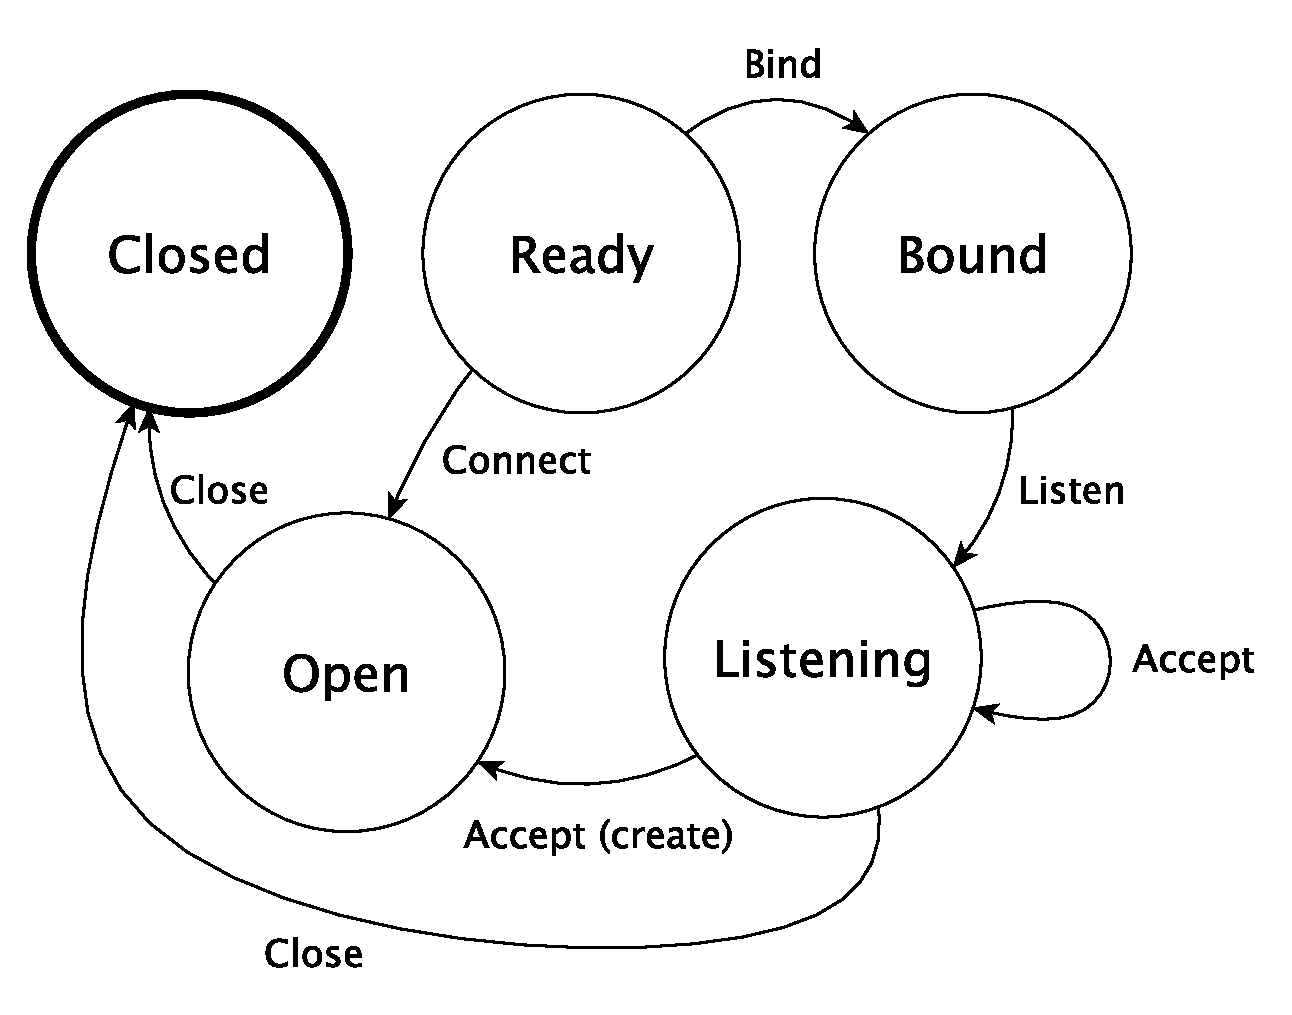
\includegraphics[width=6.5cm]{diagrams/netstate.pdf}
\end{minipage}
\end{tabular}

\small
\begin{code}[float=h, frame=single,caption={The POSIX sockets API, written
as in interface for \texttt{ST} describing how each operation affects
socket state},
label=fig:socketsiface]
data SocketState = Ready | Bound | Listening | Open | Closed

interface Sockets (m : Type -> Type) where
  Sock : SocketState -> Type

  socket : SocketType -> ST m (Either () Var) [addIfRight (Sock Ready)]
  bind : (sock : Var) -> (addr : Maybe SocketAddress) -> (port : Port) ->
    ST m (Either () ()) [sock ::: Sock Ready :-> (Sock Closed `or` Sock Bound)]
  listen : (sock : Var) ->
    ST m (Either () ()) [sock ::: Sock Bound :-> (Sock Closed `or` Sock Listening)]
  accept : (sock : Var) ->
    ST m (Either () Var) [addIfRight (Sock Open), sock ::: Sock Listening]
  connect : (sock : Var) -> SocketAddress -> Port ->
    ST m (Either () ()) [sock ::: Sock Ready :-> (Sock Closed `or` Sock Open)]
  close : (sock : Var) -> {auto prf : CloseOK st} ->
    ST m () [sock ::: Sock st :-> Sock Closed]
  remove : (sock : Var) -> ST m () [Remove sock (Sock Closed)]
  send : (sock : Var) -> String -> 
    ST m (Either () ()) [sock ::: Sock Open :-> (Sock Closed `or` Sock Open)]
  recv : (sock : Var) ->
    ST m (Either () String) [sock ::: Sock Open :-> (Sock Closed `or` Sock Open)]
\end{code}
\normalsize

Listing~\ref{fig:socketsiface} shows how these operations can be given precise
types which describe how the operations affect socket state, using \texttt{ST}.
By convention, each operation returns something with a type of the form
\texttt{Either a b}, representing the possibility of failure.
The \texttt{ST} library provides two helper functions
which allow us to write concise types for these operations:

\small
\begin{code}
addIfRight : Type -> Action (Either a b)
addIfRight ty = Add (either (const []) (\var => [var ::: ty]))

or : a -> a -> Either b c -> a
or x y = either (const x) (const y)
\end{code}
\normalsize

Note, in particular, that \texttt{accept} explicitly creates a new socket
specifically for processing an incoming connection, keeping the existing
socket in a \texttt{Listening} state. This could allow, for example, 
processing an incoming connection in a different thread.

For example, we could write an ``echo'' server which repeatedly accepts
an incoming connection from a client, and echoes a message back to the
client. We can define a function \texttt{echoServer} which accepts connections
on a \texttt{Listening} socket:

\small
\begin{code}
echoServer : (ConsoleIO m, Sockets m) => (sock : Var) -> 
             ST m () [Remove sock (Sock {m} Listening)]
\end{code}
\normalsize

Then, before we start up \texttt{echoServer}, we need to create a socket, bind
it to a port, then begin listening for incoming connections. Each of these
operations could fail, so we include pattern matching alternatives to clean
up the resources if necessary:

\small
\begin{code}
startServer : (ConsoleIO io, Sockets io) => ST io () [] 
startServer = do Right sock <- socket Stream        | Left err => pure () 
                 Right ok <- bind sock Nothing 9442 | Left err => remove sock
                 Right ok <- listen sock            | Left err => remove sock
                 echoServer sock
\end{code}
\normalsize

We can begin writing \texttt{echoServer} as follows, accepting a connection
or cleaning up the resources and returning if \texttt{accept} fails:

\small
\begin{code}
echoServer sock = 
  do Right new <- accept sock | Left err => do close sock; remove sock
     ?rest
\end{code}
\normalsize

Checking the type of \texttt{?rest} here shows us that we have a 
\texttt{new} socket, which is \texttt{Open} and therefore ready to communicate
with the client, as well as \texttt{sock} which remains listening for new
connections:

\small
\begin{code}
rest : STrans m () [new ::: Sock Open, sock ::: Sock Listening]
                   (\result1 => [])
\end{code}
\normalsize

\subsection{Asynchronous Programming with Threads}

\label{sect:async}

In \texttt{ST}, resources are linear, in that there is exactly one reference
to each, and once a resource has been overwritten the old value is no longer
available. So, if we spawn a thread, we need to consider how to preserve
linearity, and maintain only one reference to each resource.
Listing~\ref{fig:asynciface} shows one way to do this, where the
\texttt{fork} function takes a thread described in \texttt{STrans}, and
a proof that the forked thread uses a subcontext of the parent thread.
Then, the parent thread keeps only the resources which are not used by
the child thread.

\small
\begin{code}[float=h, frame=single,caption={An interface supporting
asynchronous programming, dividing resources between a child
and a parent thread},
label=fig:asynciface]
interface Conc (m : Type -> Type) where
  fork : (thread : STrans m () thread_res (const [])) ->
         {auto tprf : SubCtxt thread_res all} ->
         STrans m () all (const (kept tprf)) 
\end{code}
\normalsize

An implementation of \texttt{Conc} then needs to divide the resources
appropriately. We can achieve this with \texttt{dropSubCtxt} (to remove
the subcontext from the current thread, returning the environment) and
\texttt{runWith} (to pass that environment to the spawned thread):

\small
\begin{code}
implementation Conc IO where
  fork thread = do threadEnv <- dropSubCtxt
                   lift (spawn (do runWith threadEnv thread
                                   pure ()))
                   pure ()

\end{code}
\normalsize

The Idris library defines \texttt{spawn} to create a new thread. It
returns a process identifier, to allow communication between threads, but
we leave communication between threads for future work.

\subsection{Managing Sessions: A Random Number Server}

\label{sect:randserver}

In the turtle graphics example, we implemented a high level
graphics API in terms of lower level drawing operations. Similarly, we can
implement a high level network application protocol in terms of sockets.
Listing~\ref{fig:randiface} shows an interface for a server which replies
to requests from a client for a random number within a bound. 

\small
\begin{code}[float=h, frame=single,caption={An interface for a server which
returns random numbers within a given bound},
label=fig:randiface]
data SessionState = Waiting | Processing | Done

interface RandomSession (m : Type -> Type) where
  Connection : SessionState -> Type
  Server : Type

  recvReq : (conn : Var) ->
    ST m (Maybe Integer) [conn ::: Connection Waiting :->
                           \res => Connection (case res of
                                                    Nothing => Done
                                                    Just _ => Processing)]
  sendResp : (conn : Var) -> Integer ->
             ST m () [conn ::: Connection Processing :-> Connection Done]
  start : ST m (Maybe Var) [addIfJust Server]
  quit : (srv : Var) -> ST m () [Remove srv Server]
  done : (conn : Var) -> ST m () [Remove conn (Connection Done)]
  accept : (srv : Var) ->
           ST m (Maybe Var) [srv ::: Server, addIfJust (Connection Waiting)]
\end{code}
\normalsize

The interface defines two types:

\begin{itemize}
\item \texttt{Connection}, which is the current state of a session with
a client. A session is either \texttt{Waiting} for the client to send
a request, \texttt{Processing} the request from the client, or \texttt{Done}
and ready to close.
\item \texttt{Server}, which is the type of a server which processes
incoming client requests.
\end{itemize}

Overall, a server listens for an incoming request from a client, 
and when it receives a request, it initialises a session with the client
and continues waiting for further incoming requests. In a session, we can
call one of:

\begin{itemize}
\item \texttt{recvReq}, which, if we're in the \texttt{Waiting} state,
receives a request from a client, and if it is valid moves into the
\texttt{Processing} state.
\item \texttt{sendResp}, which, if we're in the \texttt{Processing} state,
sends a random number within the given bound. Note that \texttt{sendResp}
itself is intended to do the work of generating the random number.
\item \texttt{done}, which closes the session and removes the \texttt{Connection}
state.
\end{itemize}

To implement a random number server, we'll use this interface, as well
as \texttt{ConsoleIO} for console logging, and \texttt{Conc} to process
requests asynchronously. To avoid repetition in every function signature,
Idris provides a notation to allow us to state that every function in a
block is constrained by the same interfaces:

\small
\begin{code}
using (ConsoleIO m, RandomSession m, Conc m)
\end{code}
\normalsize

We implement a session with \texttt{rndSession} which, given a
\texttt{Connection} in the \texttt{Waiting} state will process a client
request and eventually delete the connection, using \texttt{recvReq},
\texttt{sendResp} and \texttt{done}:

\small
\begin{code}
rndSession : (conn : Var) -> ST m () [Remove conn (Connection {m} Waiting)]
\end{code}
\normalsize

The main loop of the server calls \texttt{accept} to receive an incoming
connection. If it fails, it reports an error. Otherwise, it uses
\texttt{fork} to process the incoming connection in a separate thread.
The resources are divided between \texttt{rndSession} (whose type states that
it receives the \texttt{Connection} variable) and the parent thread, which
retains the \texttt{Server} variable:

\small
\begin{code}
rndLoop : (srv : Var) -> ST m () [srv ::: Server {m}]
rndLoop srv = do Just conn <- accept srv | Nothing => putStr "accept failed\n"
                 putStr "Connection received\n"
                 fork (rndSession conn)
                 rndLoop srv
  
rndServer : ST m () []
rndServer = do Just srv <- start | Nothing => putStr "Can't start server\n"
               rndLoop srv; quit srv
\end{code}
\normalsize

Finally, we can implement the interface using composite resources for both
the \texttt{Connection} and the \texttt{Server}. Each one carries a seed
for the random number generator, and a socket for receiving incoming
connections. In the case of \texttt{Connection}, the socket will be in a
different state depending on the current state of the session. In
particular, once the session is \texttt{Done}, the socket will need to be
\texttt{Closed}.

\small
\begin{code}
implementation (ConsoleIO m, Sockets m) => RandomSession m where
  Connection Waiting = Composite [State Integer, Sock {m} Open]
  Connection Processing = Composite [State Integer, Sock {m} Open]
  Connection Done = Composite [State Integer, Sock {m} Closed]
  Server = Composite [State Integer, Sock {m} Listening]
  ...
\end{code}
\normalsize

% The complete code for this and the previous examples is available as
% supplementary material, and will be made available online.

%\section{Discussion}

\section{Related Work}

This paper builds on previous work on algebraic effects in
Idris~\citep{brady-eff2013,brady-tfp14}, and the implementation of
\texttt{STrans} follows many of the ideas used in these earlier
implementations. However, this earlier work had several limitations, most
importantly that it was not possible to implement one effectful API in
terms of others, and that it was difficult to describe the relationship
between separate resources, such as the fact that \texttt{accept} creates
a new resource in a specific initial state. The work in the present paper is
influenced in particular by previous work on Separation Logic, Linear Types 
and Session Types, and has connections with other type systems and tools
for formal verification. In this section we discuss these and other
connections.

\emph{\textsf{Separation Logic and Indexed Monads:}}
%
The representation of state transition systems using dependent types owes much
to Atkey's study of indexed monads~\citep{atkey-param}, and McBride's
implementation of dynamic interaction in Haskell~\citep{mcbride-kleisli}.  The
state transitions given by operations in \states{}, like in this previous
work on indexed monads, are reminiscent of Hoare Triples~\citep{hoarelogic}. 
Separation Logic~\citep{reynolds2002}, an extension of Hoare Logic, 
permits local reasoning by allowing a heap to be split into two disjoint
parts, like the \texttt{call} function in
\states{}. This has previously been implemented as Ynot, an axiomatic extension
to Coq~\citep{ynot08}. 
Separation Logic allows us to reason about the state of a program's heap.  The
key distinction between this previous work and \states{} is that we reason
about individual resources, such as files and network sockets, rather than
about the entire heap, and list these resources in a context.
While Separation Logic can prove more complex properties, our
approach has a clean embedding in the host language, which
leads to readable types and, because resources are combined in predictable
ways, minimises the proof obligations for the programmer. Indeed, the examples
in Section~\ref{sect:examples} require \emph{no} additional effort
from the programmer to prove that resources are used correctly.

% \citep{Chlipala2015}

\emph{\textsf{Linear Types:}}
%
Indexed monads, as used in \states{}, are a way of encoding
linearity~\citep{wadler-linear,Abramsky1993} 
in a dependently typed host language. Recent work by~\citet{neelk2015}
and by~\citet{McBride2016} has shown ways of integrating linear and
dependent types, and the latter has been implemented as an experimental
extension to Idris.
Our experience has been that linear types can provide the same guarantees
as the \states{} library, but that, subjectively, they have a more ``low-level''
feel than the indexed monad approach. A particular notational inconvenience is
the need for a function which updates a linear resource to return a new 
reference to the resource, a detail which is abstracted away by the indexed
monad. Nevertheless, we hope to explore the connection further in future work.
In particular, linear dependent types may give us an efficienct
method for implementing \states{}.

\emph{\textsf{Types and State Machines:}}
%
Earlier work has recognised the importance of state transition systems
in describing applications~\citep{statecharts}.
%
In this paper, we have used \states{} to describe systems in terms
of state transitions on resources,
both at the level of external resources like network sockets and at
the application level.
The problem of reasoning about protocols has previously been
tackled using special purpose type systems~\citep{Walker2000}, by creating
DSLs for resource management~\citep{Brady2010a}, or with
Typestate~\citep{Aldrich2009,Strom1986}. In these approaches, however,
it is difficult to compose systems from multiple resources or to implement a
resource in terms of other resources.  In \states{}, we can combine resources
by using additional interfaces, and implement those interfaces in terms of
other lower level resources.

\emph{\textsf{Types for Communication:}}
%
A strong motivation for the work in the present paper is to be able to
incorporate a form of Session Types~\citep{Honda93,Honda08} into dependently
typed applications, while also supporting other stateful components.  
Session Types describe the state of a communication channel, 
and recent work has shown the correspondence between propositions and 
sessions~\citep{propositions-sessions} and how to implement this in a
programming language~\citep{Lindley2015}. 
More recently,~\citet{Toninho2016} have shown how to increase the
expressivity of multi-party session to capture invariants on data.
We expect
to be able to encode similar properties in \states{} and in doing so, be
able to encode security properties of communicating systems with
dependent types, following~\citep{Guenot2015}.
Type systems in modern programming languages, such as Rust~\citep{session-rust}
and Haskell~\citep{session-haskell}, are strong enough to support Session
Types, and by describing communication protocols in types, we expect to be able
to use the type system to verify correctness of implementations of security
protocols~\citep{gordon2003authenticity,sewell-tls}.


%Also Dijkstra Monads~\cite{Ahman2017}

\emph{\textsf{Effects and Modules:}}
%
Algebraic effects~\citep{Plotkin2009,Bauer} are increasingly being proposed as
an alternative to monad transformers for structuring Haskell
applications~\citep{KiselyovEffects,handlers2013}.
Earlier work in Idris~\cite{brady-eff2013,brady-tfp14} has used a system
based on algebraic effects to track resource state, like \states{} in
this paper. 
Koka~\cite{Leijen2017} uses row polymorphism to describe the allowed effects
of a function, which is similar to the \texttt{Context} of an \states{}
program in that a function's type lists only the parts of the overall state it
needs.

In \states{}, rather than using effects and handlers, we use
\emph{interfaces} to constrain the operations on a resource, and provide
\emph{implementations} of those interfaces. This does not have the full
power of handlers of algebraic effects---in particular, we cannot reorder
handlers to implement exception handling or other control flow---but it
does allow us to express the state transitions precisely. Indeed, we do not
want handlers to be \emph{too} flexible: for example, a handler which
implements non-determinism by executing an operation several times would
violate linear access to a resource.
%
Interfaces in Idris are similar to Haskell type classes, but with support
for \emph{named} overlapping instances. This means that we can give multiple
different interpretations to an interface in different implementations, and
in this sense they are similar in power to ML modules~\cite{Dreyer2005}.
Interfaces in Idris are first class, meaning that implementations can be
calculated by a function, and thus provide the same power as first-class
modules in 1ML~\citet{rossberg2015}.

\section{Conclusions and Further Work}

We have shown how to describe APIs in terms of type-dependent state transition
systems, using a library \states{} and evaluated the library by presenting
several diverse examples which show how \states{} can be used in practice.
In particular, we have shown how to design larger scale systems by composing
state machines both horizontally (that is, using multiple state machines in the
same function definition) and vertically (that is, implementing the behaviour
of a state machine using other lower level state machines). 

A significant strength of this approach to structuring 
programs is that state machines are ubiquitous, if implicit, in realistic APIs,
especially when dealing with external resources like surfaces on which to draw
graphics, endpoints in network communication, and databases.  The \states{}
library makes these state machines explicit in types, meaning
that we can be sure by type checking that a program correctly follows the state
machine.  As the \texttt{Sockets} interface shows, we can give precise types to
an existing API (in this case, the POSIX sockets API), and use the operations
in more or less the same way, with additional confidence in their correctness.
%
Furthermore, as we briefly discussed in Section~\ref{sect:getdata}, and 
saw throughout the paper, we can use \emph{interactive}, type-driven, program
development and see the internal state of a program at any point during
development.

Since \states{} is parameterised by an underlying computation context, which is
most commonly a monad, it is a monad transformer.  Also, an instance of
\states{} which preserves states is itself a monad, so \states{} programs can
be combined with monad transformers, and therefore are compatible with a common
existing method of organising large scale functional programs.

There are several avenues for further work.  For example, we have not discussed
the efficiency of our approach in this paper. There is a small overhead due to
the interpreter for \states{} but we expect to be able to eliminate this using
a combination of partial evaluation~\citet{scrap-engine} and a finally tagless
approach to interpretation~\citet{Carette2009}. We may also be able to use
linear types for the underlying implementation~\citet{McBride2016} using an
experimental extension to Idris.

Most importantly, however, we believe there are several applications to
this approach in defining security protocols, and verified implementation
of distributed systems. For the former, security protocols follow a clearly
defined series of steps and any violation can be disastrous, causing
sensitive data to leak.
%
For the latter, we are currently developing an implementation of Session
Types~\citet{Honda93,Honda08} embedded in Idris, generalising the random
number server presented in Section~\ref{sect:randserver}.

The \states{} library provides a generic interface for implementing a useful
pattern in dependently typed program in such a way that it is \emph{reusable}
by application developers. State is everywhere, and introduces complexity
throughout applications. Dependently typed purely functional programming gives
us the tools we need to keep this complexity under control.


\bibliography{dtp}

\end{document}

